\documentclass[a4paper,12pt]{report}
\usepackage[utf8]{inputenc}  % for danish letters
%\usepackage[T1]{fontenc}
\usepackage[british]{babel}  % language
%\usepackage[yyyymmdd]{datetime}
\usepackage{geometry}  % layout
\usepackage{titlesec} % for customizing
\usepackage{tocloft} % spacing for table of content
\usepackage{graphicx} % for added graphics
\usepackage{pdfpages}
\usepackage{amssymb}  % weird signs
\usepackage{upgreek}  % same
\usepackage{proof} % for inference rules
\usepackage{amsmath} % for inference rules array

% for tables
\usepackage{array} 
\usepackage{tipa}

%\usepackage[acronyms,toc]{glossaries}  % References, toc for shown in table of content

% Customized chapter titles
\titleclass{\chapter}{top}
\titleformat{\chapter}[hang]{\LARGE\bfseries}{\thechapter\hspace{20pt}
{\textbar}\hspace{20pt}}{0pt}{\LARGE\bfseries}

% Customized Section titles
\titleformat*{\section}{\large\bfseries}
\titleformat*{\subsection}{\normalsize\bfseries}

% bibliography
\usepackage[backend=bibtex,style=ieee]{biblatex}
\bibliography{Literature} 
\bibliography{Online} 

\title{Extending Session Types to Model Security Properties}
\author{Julie Tollund}

\begin{document}
\pagenumbering{gobble}
%\includepdf{frontpage}   // include ITU front page
\pagenumbering{roman}
\maketitle

\setlength{\cftbeforesecskip}{10pt}  % set spacing
\tableofcontents
% TODO: Glossary and Acronyms?
\clearpage

\pagenumbering{arabic}
\chapter{Introduction}
\label{chap:Introduction}
The purpose of this report, is to establish a foundation for the future thesis by the author, in regards of extending session types to model security properties with the introduction of adversaries.

In the report I will first introduce the motivation for exploring this field, as well as the current research done in the area. Secondly, I will introduce different research areas, all related to the field, and how these work together as background knowledge for the future thesis, by which I will explain further about in the final section of this report. 

\section{Motivation}
With IT becoming an ever bigger part of our lives, the need for stronger and better security measurements, has grown with it. In recent years we have seen the introduction of voting machines in the USA and a digitalisation of our hospitals here in Denmark. With this comes the importance of being able to restrict access to ensure acceptable behaviour especially in the presence of malicious adversaries where it becomes paramount. To solve this many researchers have suggested using security protocols to ensure these security guarantees. In this report I will highlight some of the research that has made it easier to program these security protocols, as it can be a complex and error prone task. 

A lot of research has gone into communication protocols in the recent years, and fields such as Session Types, has made it a lot easier to build such protocols and ensure they are correct by construction. This idea however falls apart, when we introduce an adversary, as an attacker would be able to block messages from being delivered. This creates the motivation for doing the future thesis of introducing cryptography to Session Types, and with this report, create a basic understanding of the different fields. 

Security measurements has not only been introduced through protocols, but also through physical hardware, adding another layer of authentication. The company Trusted Computing Group introduced the Trusted Platform Module (TPM), a physical chip implemented on the motherboard, that provides a safe space for generating cryptographic keys, which is now used in a lot of modern computers and as a part of the Microsoft BitLocker. The TPM will be used as case in the thesis and is therefore also presented and explained in the following report. 

%Tighter restrictions (session types - adversaries) \\
%TPM (new security measurement) \\

\section{Current research}
The project relies heavily on the research done within the field of Security protocols and Session types. A lot of research has already gone into the field of the TPM specifications, especially by Ryan, Delaune, Kremer \textit{et al.} \autocite{DBLP:conf/ifip1-7/DelauneKRS10}, and will work as a foundation for the TPM's commands and protocols. Furthermore the report will use \citeauthor{DBLP:journals/ftpl/CortierK14,} to formally model security protocols and their goals.

\section{Intended outcome}
The intended outcome of the thesis, will be to take the idea of session types and consider them in an adversarial environment. This will be done by extending session types to model properties, and
from this produce protocols that are secure by construction. Furthermore a compiler will be constructed to automate the process of producing these programs afterwards. 

\chapter{Work Done}
\label{chap:Background Study}
This section describes the work carried out so far. Most of it will be highlighting research done within the different fields, and showcasing examples of its use. The section ends in a summery of how the different fields come together, and how they can be used further in the coming thesis. 

\section{Security Protocols} % Message deduction?
Security protocols is an abstract or concrete protocol, that characterise the security related functions and applies cryptographic methods. It describes how the algorithm should be used to ensure the security and integrity of data transmitted. The security protocol is a protocol that runs in an untrusted environment, where it usually assumes channels are untrusted and participants are dishonest. In academic examples, they are often described with the Alice and Bob notation, which will also be used in the following examples. (The Dolev-Yao model) 

%A way of reason about wether a message is deductible by an adversary is through inference rules. Inference rules offers a formal analysis for proving security properties of protocols. \\ \\
%TODO: discuss how Inference rules and derivation sequences can be used 

\subsection{Needham-Schroeder Protocol}
The Needham-Schroeder Public Key Protocol, was first proposed by Roger Needham and Michael Schroeder in 1978 (ref?), and will be used as a running example in this and the following two sections. %and is one of the two key transport protocols intended for an insecure network. 

The Needham-Schroeder Public Key Protocol can be illustrated by the before mentioned Alice and Bob notation in the following way, as done by \citeauthor{DBLP:journals/ftpl/CortierK14}

\begin{center}
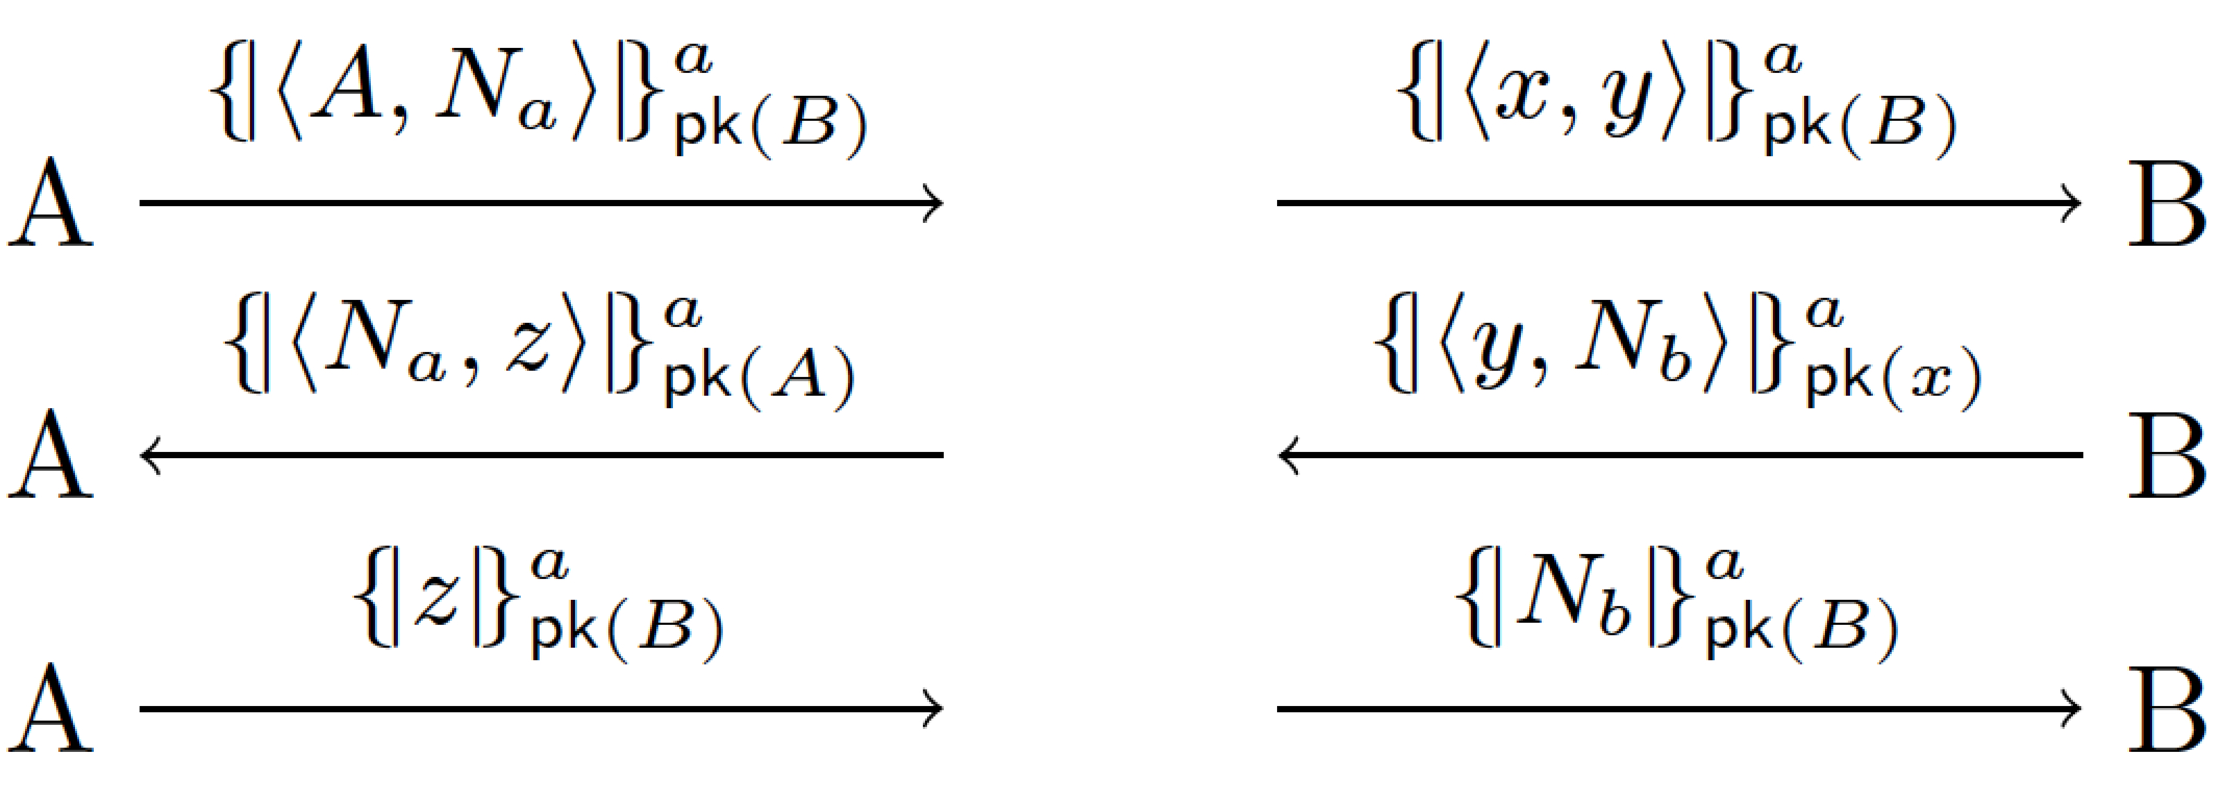
\includegraphics[width=0.7\textwidth, angle=0]{Graphics/NS_Protocol.pdf}
\end{center}

The A and B each represent Alice and Bob, while the arrows indicates the direction of the sent and received messages, by which are illustrated above each line. The notation $\{| m |\}^a_{pk(B)}$ denotes that the message \textit{m} is created with an asymmetric encryption of Bob's public key, while the $\langle m_1, m_2 \rangle$ illustrates a pairing, so a concatenation of the two messages. 
\\ \\The cap left between the two participants, is to illustrate the challenge of this protocol, and will be addressed later in the report. 

\iffalse
A -> B : m  			= Alice sends Bob a message
Notation {|m|}^a_pk(B) 	= asymmetric encryption of m with Bob's public key. 
<m1, m2>				= pairing, i.e. concatenation of the two messages
A, B					= Their identities
N_a					= nonce (number used once - fresh random generated each session)
First 					= Alice sends her identity and nonce, encrypted with Bob's public key

Bob then decrypts and check that it is well-formed.
This mechanism of sending someone an encrypted nonce and waiting for the recipient to send back this nonce is often called a challenge-response mechanism.
Alice then decrypts Bob's message, and verifies that it contains har previous N_a - proves that Bob received first message

The aim of the protocol is to guarantee mutual 'authentication' - ensures they have been communicating with the right person
Moreover, the protocol should guarantee 'confidentiality' of the nonces Na and Nb.
 - Honest execution (man in the middle attack)
\fi

\subsection{Message deduction}
TODO: Deduction rules \\
TODO: Derivation sequence

%\subsection{Examples}
%TODO: show examples of a man in the middle attack on the NS and DH protocols: \\ \\
%- Needham-Schroeder Public key protocol (now modified according to Lowe's man in the middle attack): 



\section{Applied $\pi$-Calculus}
%Short - examples of the applied $\pi$-calculus 
%\begin{itemize}
%  \item General about Applied Pi Calculus, and how it differs from pi calculus (terms; in particular for security protocols)
%  \item Examples of applied pi calculus (handshake protocol?)
%  \item ProVerif - automatic symbolic protocol verifier
%\end{itemize}

% missing link from the unformal way of Alice and Bob notation (but more convenient), to the more formal applied pi-calculus
% "The previous chapter describes how messages exchanged in cryptographic protocols can be represented as terms. In this chapter, we discuss how the protocols themselves can be modelled."
The applied pi-calculus (ref. Abadi and Fournet, 2001) is based upon the language pi-calculus, but offers a more convenient use for modelling security protocols to be specified, by allowing for a more wide variety of complex primitives. It is used for describing and analysing security protocols, as it provides a more intuitive process syntax for detailing the actions of the participants in a protocol \autocite{AplliedPiCalsulus2010}. This is done by introducing a rich term algebra for modelling the cryptographic operations used in security protocols, where function symbols represent cryptographic protocols. 

Tools such as ProVerif \autocite{ProVerif} uses a syntax closely related to the applied pi-calculus, and offers a way of automated reasoning about the security properties found in cryptographic protocols. The ProVerif tool is however not used for this report, but is mentioned as it is often used when analysing security protocols, and will most likely be used in the following thesis.\\
%- The properties of these primitives are modelled by equations \\ 

%"The applied pi calculus (...) is a language for describing concurrent processes and their interactions". \\
\subsection{Syntax}
As mentioned, the applied pi-calculus is not restricted to communication names, but offers processes where they output terms representing messages instead. The applied pi-calculus has two two types of process, the \textit{plain} and \textit{extended} processes. First we describe the grammar for the \textit{plain} process, as shown below (fig. ref?).:  %(by \citeauthor{AplliedPiCalsulus2010}): 
\begin{center}
	\begin{tabular} { l l }
 		$P,\ Q,\ R$ ::= & plain processes \\ 
 		\quad $|$ 0 & null process \\  
 		\quad $|$ $P\ |\ Q$ & parallel composition \\
 		\quad $|$ !$P$ & replication \\
		\quad $|$ $\nu n.P$ & name restriction \\
		\quad $|$ if \textit{M = N} then \textit{P} else \textit{Q} & conditional \\
		\quad $|$ $u(x).P$ & message input \\
		\quad $|$ $\overline{u}\langle M\rangle .P $ & message output 
	\end{tabular}
\end{center}
The 0 process is the process that does nothing; $P\ |\ Q$ is the parallel composition of the processes \textit{P} and \textit{Q} executed in parallel; !$P$ is the replication of \textit{P} that allows for an infinite composition of $P\ |\ P\ |\ ...,$ which is often used for illustrating an unbound number of sessions; Name restriction $\nu n.P$ acts as a binder which generates a restricted name \textit{n} inside \textit{P}. This is often used for capturing fresh random numbers such as nonces and keys, or private channels, which we will see later when we apply it to the NS Protocol; The conditional if \textit{M = N} then \textit{P} else \textit{Q} is how we know from normal conditioning, where it behaves as \textit{P} whenever \textit{M = N} (representing equality), and as \textit{Q} otherwise; Last we have the message input and output, where $u(x).P$ expects an input on channel \textit{u} and binds it to variable \textit{x} in \textit{P}, and $\overline{u}\langle M\rangle .P $ outputs term \textit{M} on channel \textit{u} and then behaves as \textit{P}. It should be noted that message input and output will also we written as in\textit{(u, x).P} and out\textit{(u, M).P} as done by \citeauthor{DBLP:journals/ftpl/CortierK14} \\
\iffalse
Plain processes are generated by the grammar given
in Figure 5.1, where t, t1, t2, . . . range over terms, n over names, x over
variables and u is a meta-variable that stands for either a name or a
variable of channel sort. 
\fi

% Extension
Processes are extended with \textit{active substitutions} to capture the knowledge exposed to the
adversarial environment: (rewirte)
\begin{center}
	\begin{tabular} { l l }
 		\textit{A, B, C} ::= & extended processes \\ 
 		\quad $|$ \textit{P} & plain process \\  
 		\quad $|$ $A\ |\ B$ & parallel composition \\
		\quad $|$ $\nu n.A$ & name restriction \\
		\quad $|$ $\nu x.P$ & variable restriction \\
		\quad $|$ $\{ \sfrac{M}{x} \}$ & active substitution
	\end{tabular}
\end{center}
With \textit{active substitution} we allow for \textit{M} to be available in the environment through the 'handle' \textit{x}. In other words, \textit{M} can now be replaced by \textit{x} in every process it is related to, and is only controlled by the variable restriction, i.e. $\nu x.(\{\sfrac{M}{x}\}\ |\ P)$ is exactly the same as $x$ = $M$ in $P.$\\ 
%Terms

With terms we use function symbols to capture primitives such as encryption or decryption used by cryptographic protocols. It should be noted that functions with arity 0 are what we define as constants.
For terms we apply function symbols to names, variable and other terms as such: 
\begin{center}
	\begin{tabular} { l l }
 		L, M, N, T, U, V ::= & terms \\ 
 		\quad $|$ a, b, c,...,k,...,m, n,..,s & names \\  
 		\quad $|$ x, y, z & variables \\
 		\quad $|$ g(M$_{1}$,..,M$_{l}$) & function application
		%\caption{Fig. 1.1}
		%\label{tbl:excel-table}
	\end{tabular}
\end{center}
TODO: description (maybe first)

\subsection{Re-visiting the Needham-Schroeder Protocol}
Having established an understanding og the applied pi-calculus and its grammar, we now use it model the previously mentioned Needham-Schroeder public key protocol.\\

To make this distinction explicit we parametrize the processes representing the initiator and responder with the keys of the agents who execute the role. (rewrite!!):
\begin{center}
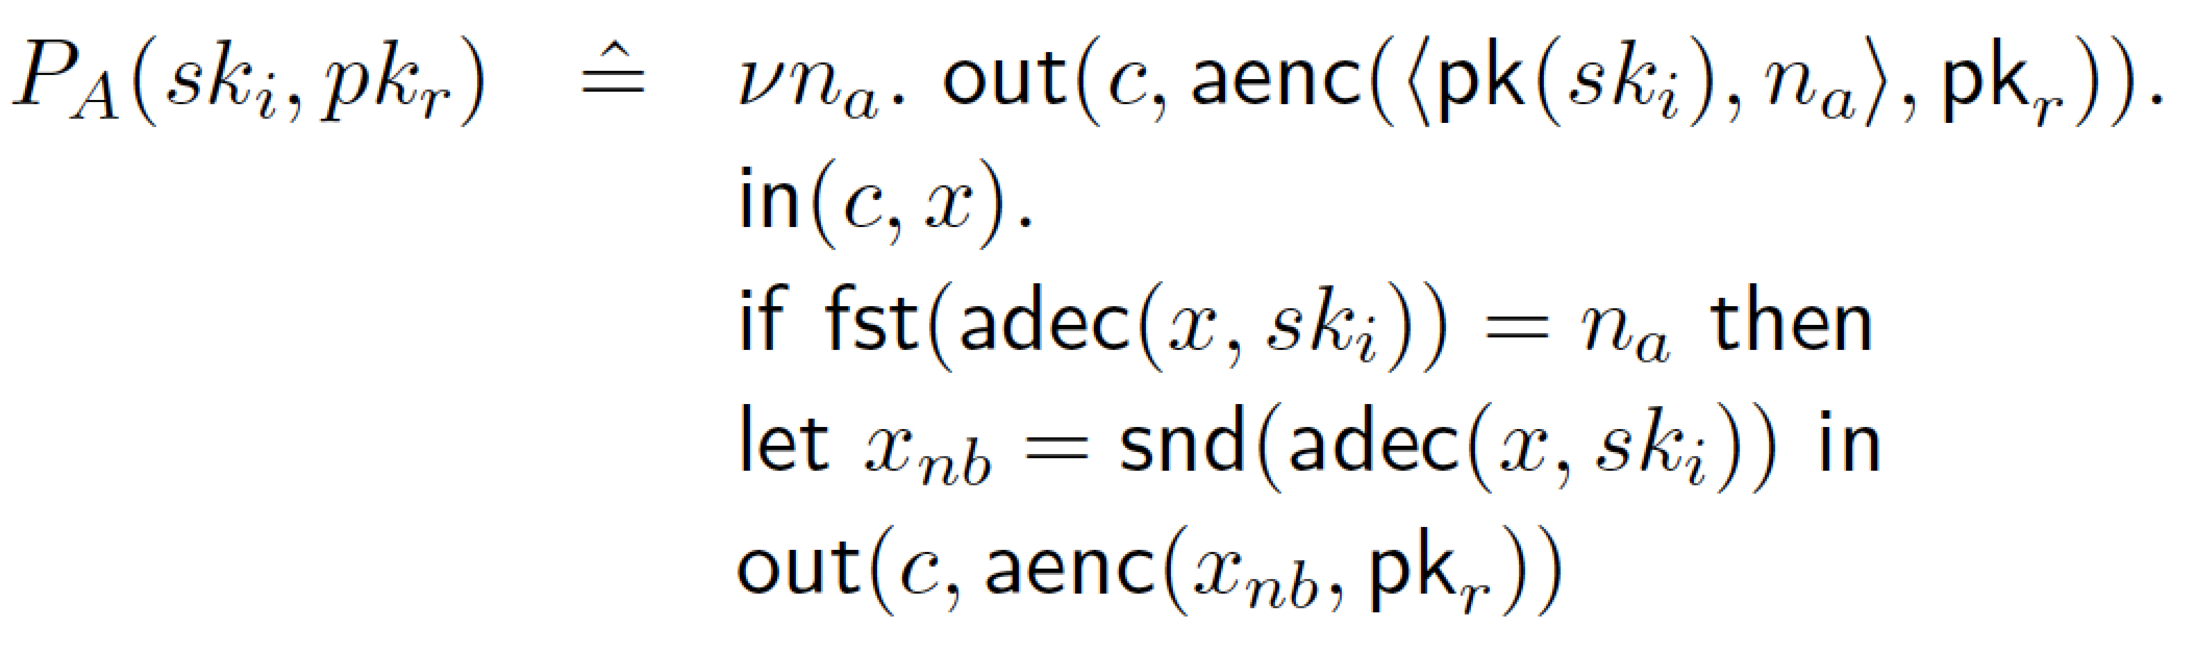
\includegraphics[width=0.65\textwidth, angle=0]{Graphics/P_A.pdf}
\end{center}
First Alice generates a fresh random nonce and binds it to \textit{n$_a$}, the process then continues to output the first message of an asymmetric encryption on channel \textit{c}. Next she waits for a input message on the same channel, and binds the message to variable \textit{x}. She then checks wether the message matches her previously sent nonce \textit{n$_a$} shown as the conditional. For readability the \textit{x} is then bound to a local variable \textit{n$_xb$}, representing the nonce received by the sender (Bob). Last she sendt out a message again on channel c. \\

\noindent The dual of the process can now be modelled from the responders point of view:
\begin{center}
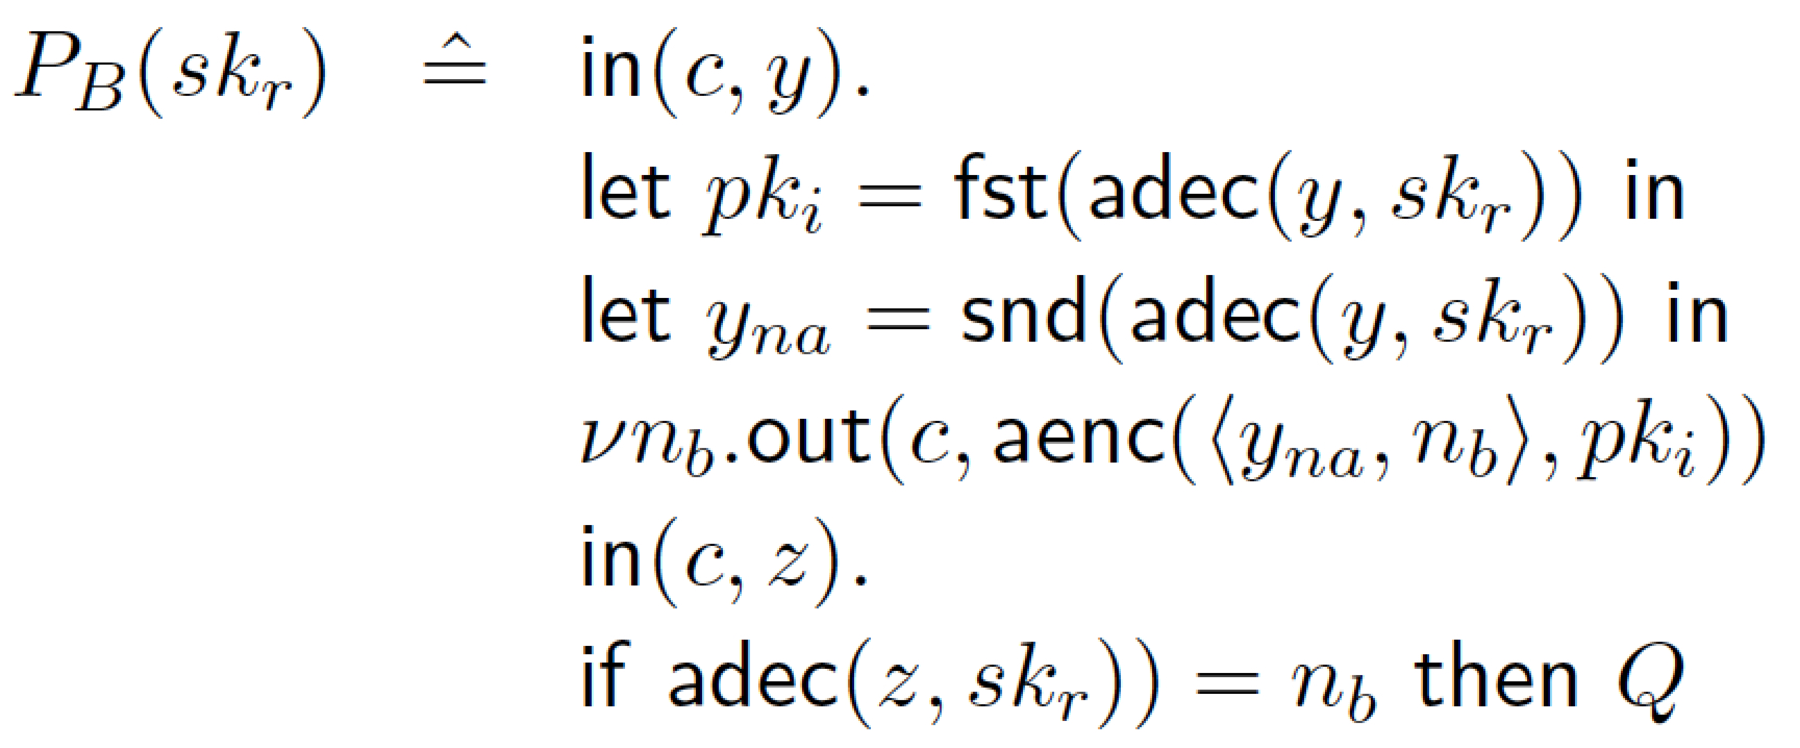
\includegraphics[width=0.55\textwidth, angle=0]{Graphics/P_B.pdf}
\end{center}

\noindent Combining the two processes, we are able to model the Needham-Schroeder public key protocol as a whole: 
\citeauthor{DBLP:journals/ftpl/CortierK14} (Describe P$_{A}$ and P$_{B}$ first):
\begin{center}
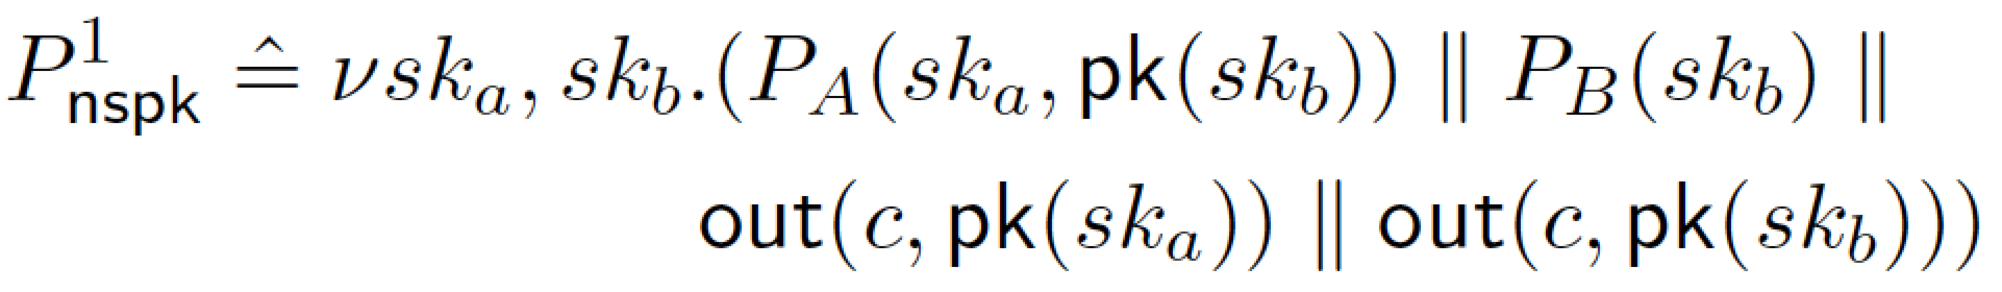
\includegraphics[width=0.6\textwidth, angle=0]{Graphics/P1_nspk.pdf}
\end{center}
This however represent the naive model of the protocol, so to add the Lowe fix, as mentioned earlier i then report, we add the identity to the encryptions: (TODO: needs further explanation)
\begin{center}
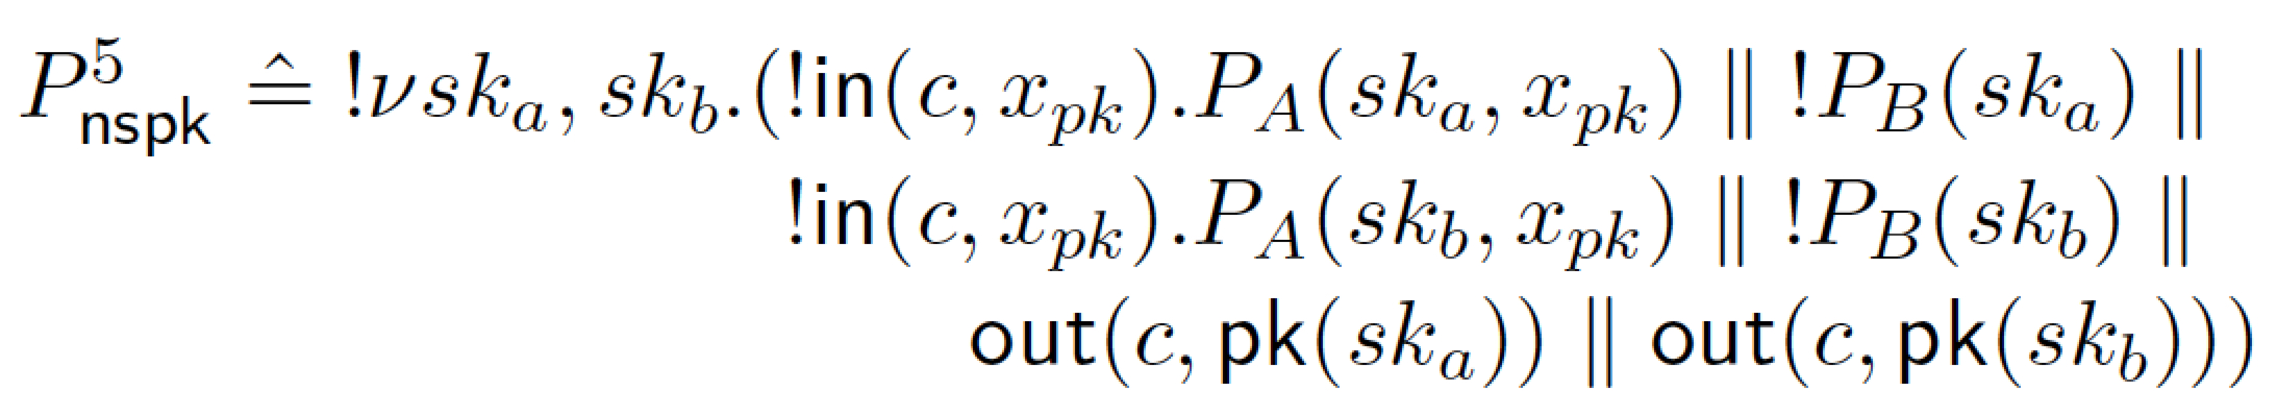
\includegraphics[width=0.6\textwidth, angle=0]{Graphics/P5_nspk.pdf}
\end{center}
TODO: smooth transition to the next chapter + don't forget reference to article!


% Extra
% Handshake protocol
\iffalse
First of, we look at the simple Handshake protocol used for setting the parameters for communication between two devices, such as the old dial-up modem or when connecting to a USB.  \\
Handshake protocol with applied pi-calculus as illustred by \citeauthor{AplliedPiCalsulus2010}:
\begin{center}
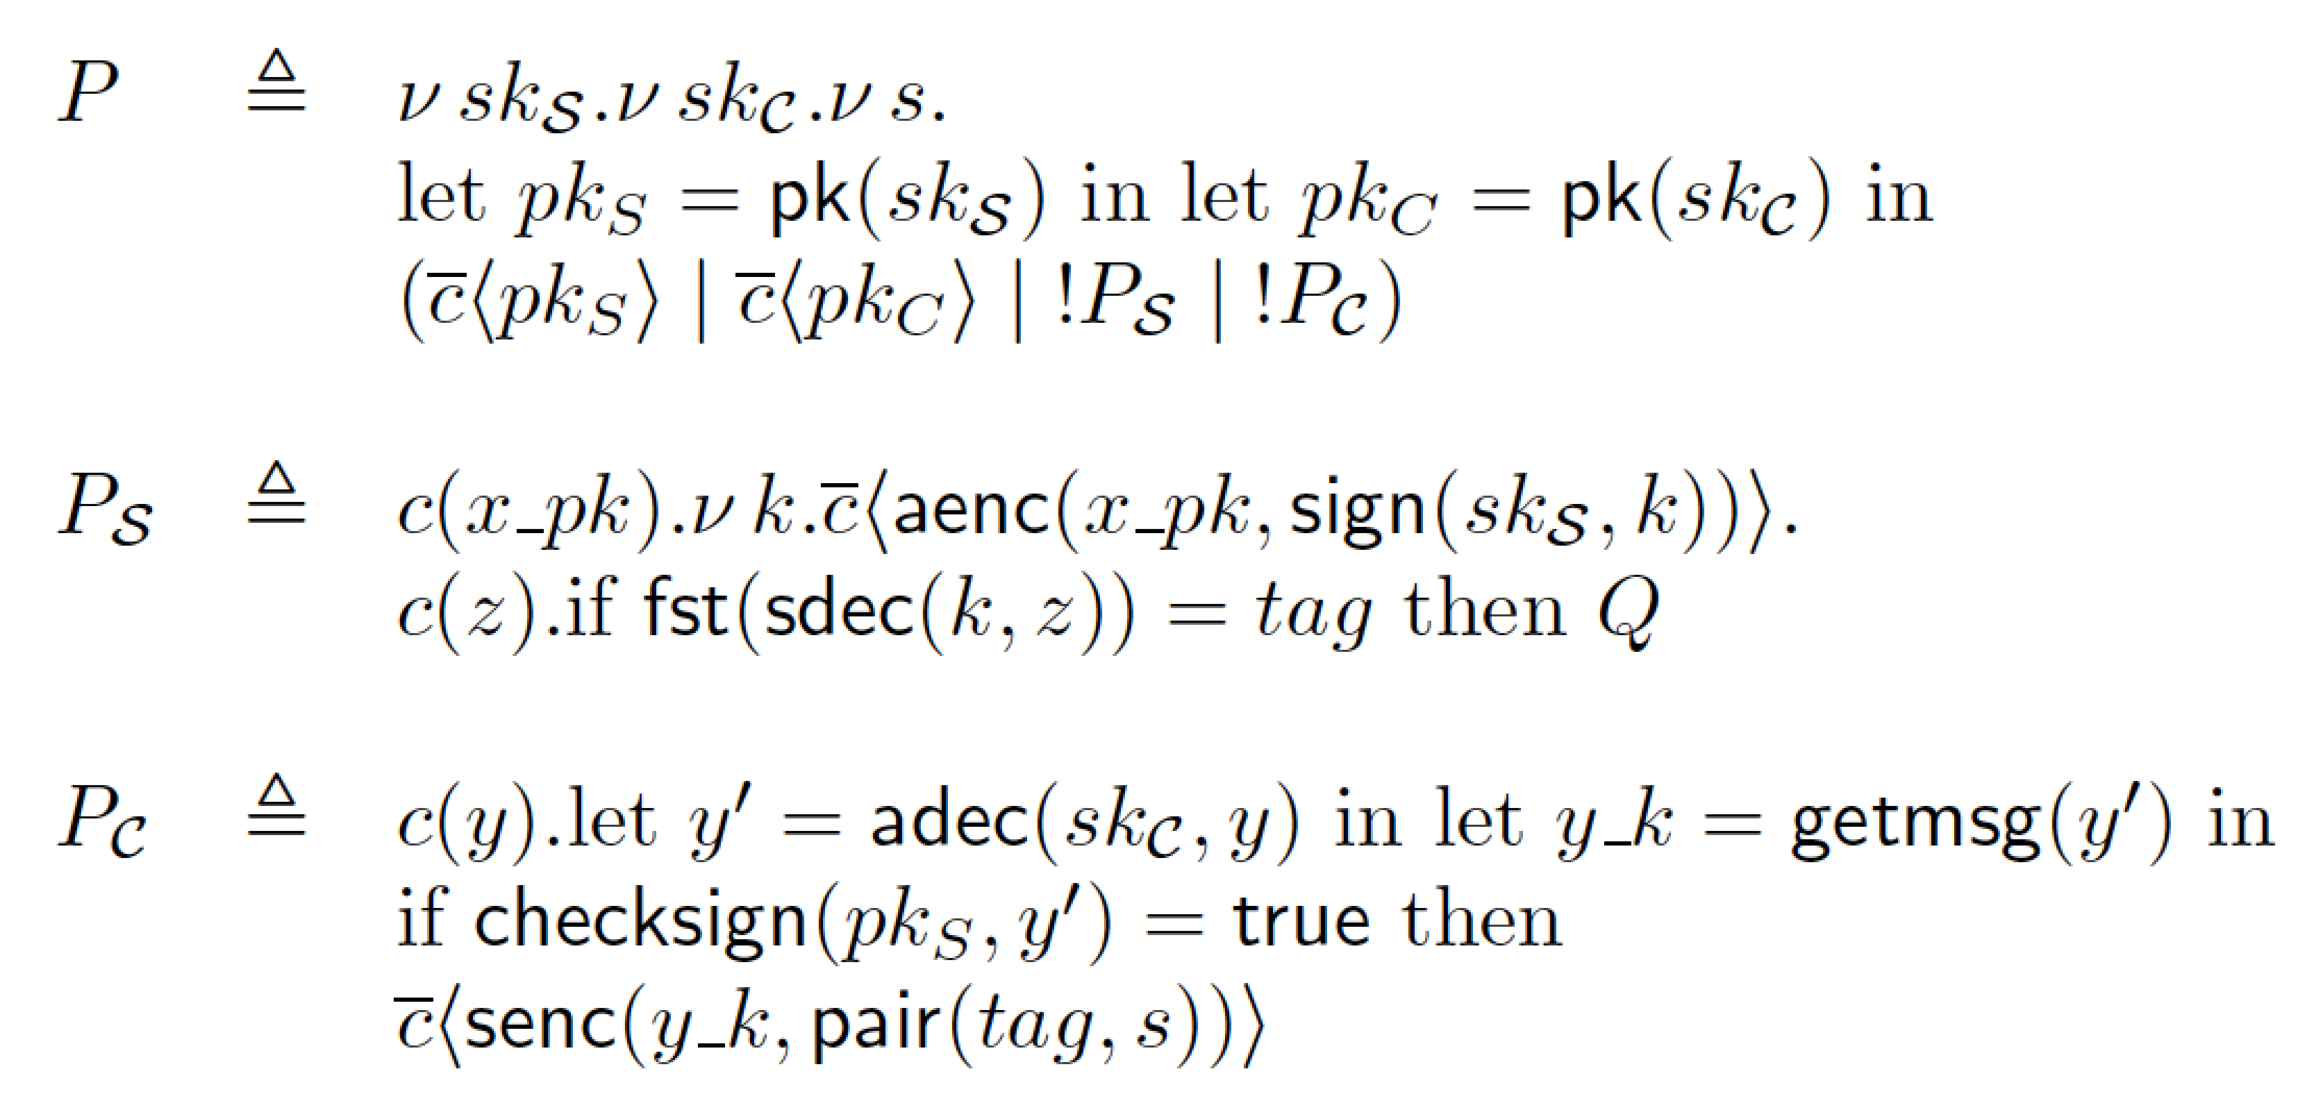
\includegraphics[width=0.75\textwidth, angle=0]{Graphics/Handshake.pdf}
\end{center}
\fi

\section{Session Types (and choreography programming)}
TODO: Description of session types and what they are used for

\subsection{Research within the field}
TODO: 

\subsection{Global Session Types}
TODO:  + Examples
\section{TPM}
\begin{itemize}
  \item Description of the TPM - what it is, and what it's used for
  \item Examples of TPM commands
\end{itemize}

The Trusted Platform Module (TPM) is a specialised chip that stores RSA encryption keys specific for the host system for hardware authentication. It is used as a component on an endpoint device and is used for the Windows BitLocker.
The TPM contains an RSA key pair called the Endorsement Key (EK), together with an owner-specified password. The Storage Root Key (SRK) is created when a user or administrator takes ownership of the system (rephrase), and works in a tree like structure to store TPM generated RSA keys used. \\ \\
The TPM offers two authorisation sessions:
\begin{itemize}
  \item Object Independent Authorisation Protocol (OIAP)
  \item Object Specific Authorisation Protocol (OSAP)
\end{itemize}
The OIAP creates a session that can manipulate any object, but will only work with certain commands. The OSAP creates a session that can only manipulate a specific object, specified at the session start.
\section{Evaluation}
\begin{itemize}
  \item How they all come together
  \item Examples of TPM commands with session types
\end{itemize}

\chapter{Future Plan}
\label{chap:Future Plan}
Farewell

\clearpage
\pagenumbering{roman}
\appendix

\nocite{*}  % for no references but still print
\printbibliography[title={References},nottype=misc]
\printbibliography[title={Online references},type=misc]
% \citeauthor{name}
% \autocite{name}
% \textquote{\textit{quote}}\autocite

\end{document}